\documentclass[aspectratio=169]{beamer}
\usepackage[utf8]{inputenc}
\usepackage{graphicx}
\graphicspath{./}
\usepackage{pslatex}
\usepackage[greek.polutoniko,hebrew,english]{babel}
\usepackage{cjhebrew}
\usepackage{multicol}
\usetheme{Berkeley}
\usecolortheme{albatross}

\title{Nomina Sacra}
\author{Kenneth Gardner}

\begin{document}

\newcommand{\lord}{L{\scriptsize ORD}}
\newcommand{\yhwh}{Y{\scriptsize HWH}}

\makeatletter
\newcommand*{\textoverline}[1]{$\overline{\hbox{#1}}\m@th$}
\makeatother

\maketitle

\begin{frame}
  Ways to discern a Christian manuscript from, say, a Jewish manuscript:\pause
  \begin{itemize}
	\item Christians used the codex.\pause
	\item Christians use \emph{nomina sacra}.
  \end{itemize}
\end{frame}

\begin{frame}
  \emph{Nomina sacra} were abbreviations for sacred names.
  They were present in virtually all, if not all, Christian manuscripts.
\end{frame}

\begin{frame}
  \selectlanguage{greek}
  \textoverline{PR} <hm~wn <o >en to~is o>urano~is\\
  <agiasj'htw t`o >'onoma sou,\\
  >elj'etw <h basile'ia sou,\\
  genhj'htw t'o j'elhm'a sou,\\
  <ws >en o>uran~w| ka`i >ep`i t~hs g~hw;\\
  t`on >'arton <hm~wn t`on >epio'usion d`os <hm~in s'hnmeron;\\
  ka`i >'afes <hm~in t`a >ofeil'hmata <hm~wn,\\
  <ws ka`i <hme~is >af'hkamen to~is >ofeil'etais <hm~wn;\\
  ka`i m`h e>isen'egkhs <hm~as e>is peirasm'on,\\
  >all`a <r~usai <hm~as >ap`o to~u ponhro~u.
  \selectlanguage{english}
\end{frame}

\begin{frame}
  Common \emph{nomina sacra} in Greek were:\pause \selectlanguage{greek}
  \begin{itemize}
	\item K'urios,\selectlanguage{english} \textoverline{KC}\pause\selectlanguage{greek}
	\item Qrist'os, \textoverline{QR}, \textoverline{Q}\selectlanguage{english}\textoverline{C}\selectlanguage{greek}\pause
	\item J'eos, \textoverline{J}\selectlanguage{english}\textoverline{C}\pause\selectlanguage{greek}
	\item M'hthr, \textoverline{MR}\pause
	\item U<i'os, \textoverline{UI}\selectlanguage{english}\textoverline{C}\pause\selectlanguage{greek}
	  \item Swt'hr, \selectlanguage{english}\textoverline{C}\selectlanguage{greek}\textoverline{R}\pause
	\item Dau'id, \textoverline{DAD}
	  \selectlanguage{english}
  \end{itemize}
\end{frame}

\begin{frame}
  These marks appear in other languages too.
  Latin has abbreviations like \textoverline{IHS}.
\end{frame}

\begin{frame}
  The Jews had their own traditions to designate the Tetragrammaton.
  It could be written with four dashes, a different color, the first and last character then space markers in between, or several other conventions.
  Though these served the same purpose, they probably aren't the root of the \emph{nomina sacra}.
\end{frame}

\begin{frame}
  \emph{Nomina sacra} are probably why we write a reference to \yhwh\ as \lord .
\end{frame}

\begin{frame}
  \begin{multicols}{2}
	The abbreviation X-mas goes back to the beginning of the convention.
	``Christ'' began abbreviated as \textoverline{XP}.
	The elements were more often combined.
  \columnbreak
	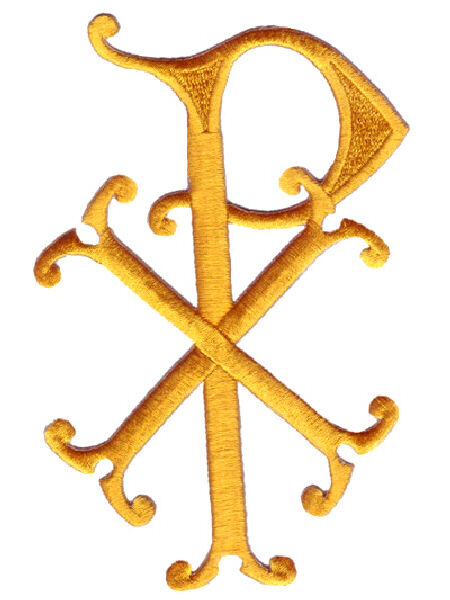
\includegraphics[scale=.5]{chirho.jpg}
  \end{multicols}
\end{frame}

\begin{frame}
  \textoverline{XP} is indeclinable.
  This leaves sentences ambiguous.
  So later, it was changed to include the ending: \textoverline{XC} for \textgreek{Qrst'os}, \textoverline{XY} for \selectlanguage{greek}Qristo~u,\selectlanguage{english} and so on.
\end{frame}

\begin{frame}
  It probably began as an outgrowth of numerology in the early Church.
  Numbers were written with an overline, so that \textoverline{IA} was 11.
  After the \emph{nomina sacra} it began to be written as \textgreek{ia'}.
\end{frame}

\begin{frame}
  This effects our approach to the text in a couple of different ways.
  First, like the red letters or quotation marks, it boxes in our range of interpretation.
\end{frame}

\begin{frame}
  It also reveals what early Christians thought of certain terms.
  Both ``Mary'' and ``David'' are uniformly abbreviated.
  This indicates special veneration for their persons.
\end{frame}

\begin{frame}
  In the previous two senses, the \emph{nomina sacra} act as a commentary.
  Accents in Greek and \emph{nikkud} in Hebrew do the same thing.
  They are not part of the originally written text, but they become part of the transmission outlining what the accepted understanding of the text is.
\end{frame}

\begin{frame}
  It also has aethetic implications.
  We print Bibles with two columns.
  It sets the text apart in our minds and culturally.
  The \emph{nomina sacra} are such a universal convention that they also mark the text as special.
\end{frame}

\begin{frame}
  There are no Bibles that replicate these in English, and so we have lost some of the meaning that was included with textual transmission.
  No \emph{propositional} truths are lost, but it certainly does impact the atmosphere and feel of the text.
  Not all truths are propositional.
\end{frame}

\end{document}
